\documentclass{article}

% if you need to pass options to natbib, use, e.g.:
%     \PassOptionsToPackage{numbers, compress}{natbib}
% before loading neurips_2018

% ready for submission
% \usepackage{neurips_2018}

% to compile a preprint version, e.g., for submission to arXiv, add add the
% [preprint] option:
%     \usepackage[preprint]{neurips_2018}

% to compile a camera-ready version, add the [final] option, e.g.:
\usepackage[preprint]{nips_2018}

% to avoid loading the natbib package, add option nonatbib:
%     \usepackage[nonatbib]{neurips_2018}

\usepackage[utf8]{inputenc} % allow utf-8 input
\usepackage[T1]{fontenc}    % use 8-bit T1 fonts
\usepackage{hyperref}       % hyperlinks
\usepackage{url}            % simple URL typesetting
\usepackage{booktabs}       % professional-quality tables
\usepackage{amsfonts}       % blackboard math symbols
\usepackage{nicefrac}       % compact symbols for 1/2, etc.
\usepackage{microtype}      % microtypography

\usepackage[english]{babel}
\usepackage{amsmath} 
\usepackage{lastpage}
\usepackage{enumerate}
\usepackage{lineno}
\usepackage{caption}
\usepackage[T1]{fontenc}
\usepackage{systeme}
\usepackage{amsmath,amssymb,amsthm,mathrsfs,latexsym,tikz,url}
\usepackage{epigraph,graphicx}
\usepackage{listings}
\usepackage{listingsutf8}
\usepackage{color}
\usepackage{float}

\usepackage{hyperref}
\hypersetup{
	colorlinks=true,
	linkcolor=blue,
	filecolor=magenta,      
	urlcolor=cyan,
}
\urlstyle{same}

\lstset{frame=tb,
	language=Python,
	aboveskip=3mm,
	belowskip=3mm,
	showstringspaces=false,
	columns=flexible,
	basicstyle={\small\ttfamily},
	numbers=none,
	numberstyle=\tiny\color{gray},
	keywordstyle=\color{blue},
	commentstyle=\color{dkgreen},
	stringstyle=\color{mauve},
	breaklines=true,
	breakatwhitespace=true,
	tabsize=4
}


\setlength{\parindent}{0.0cm}
\setlength{\parskip}{0.1cm}


\title{DD2424 Group 118: \\ The mechanisms, powers and limitations of some Data Augmentation techniques}

\author{%
  Anton Stråhle \And Jan Alexandersson \And Fredrika Lundahl}

\begin{document}
	
\maketitle

\begin{abstract}

300 words maximum, currently 100 words

To obtain good results in deep learning the quality and quantity of the data is crucial. A smart and cheap way of increasing and improving the available data is data augmentation. In this project we have tried different augmentation techniques such as mix up, Fourier transforms and more ordinary manipulations such as rotations and brightness adjustments on top of a decently performing CNN as well as some experiments on Resnet and Mobilenet. We have tried to see during which circumstances the augmentations have effect, and how big that effect is. The data set used consist of about 25 000 colored images of 200 bird species, mostly from the United States. The data has further been divided into subsets of different size and difficulty. Our results show that the Fourier transform does not seem to have a positive effect on the accruacy. We also see that basic data augmentations techniques seem to increase the performance, whilst MixUp does not seem to impact the performance in a positive manner, in all examined cases.


\end{abstract}

\section{Introduction}

0.5-0.75 pages

\textit{Describe the problem you are working on and why it is important. Then also briefly describe what you did and give an overview of your results.}

One of the major drawbacks of supervised learning is the need of immense amounts labeled data, producing such in the quantity needed for optimal results can be both costly and extremely time demanding, if even possible at all, which may be the case with medical data where only a limited number of known and active cases may exist.  (Shorten \& Khoshgoftaar, 2019). 

Data augmentation provides a partly solution to this issue when it comes to image classification and after being briefly introduced to some data augmentation techniques during the lectures we wanted to explore this topic further and investigate the payoff (or lack of) from some data augmentation techniques as well as getting an understanding of when it is worth the effort. We are interested in interpretability and have used this project to in an experimental way find the how, when and whys. 

Our main focus is to try out mixup and Fourier transformation in practice, but we have also chosen to apply some more standard augmentations such as rotations simple adjustments to have something to compare with.

To clarify, our project does not aim to obtain the highest possible testing accuracy but rather aim to show the impact of data augmentations 
on the accuracy. 

For our experiments we created a basic CNN architechture as well as implemented a fully trained version of ResNet50 in order to also examine the effects on data augmentations techniques in the case of transfer learning.

To create different settings we divided the original data into different subsets with different sizes and characteristics, some random and some more targeted such as birds with bright colors, some with very little training images per species and some with more.

\section{Related Work}

\subsection{Basic Data Augmentation}

\href{https://link.springer.com/article/10.1186/s40537-019-0197-0}{A survey on Image Data Augmentation for Deep Learning} by Shorten \& Khoshgoftaar is a profound survey paper providing guidelines for different data augmentations and applications. The power of data augmentations is a red line throughout the text but the authors also emphasize the need of choosing the right augmentations for the specific dataset, and points out that in situations with very little data, augmentations may even lead to further overfitting, which is the direct opposite of its purpose. This is something we would like to investigate further, as being aware of problems may be as important as advantages.


\subsection{Mixup}

The concept of Mixup was introduced by \href{https://arxiv.org/pdf/1710.09412.pdf}{Zhang et al}(2018) and was published as a conference paper at ICLR 2018. Mixup is really fascinating because of its' creativeness and ability to improve performance while being very simple. As a motivation to the augmentation the authors mention that networks often pay too much attention to contradictory cases and tend to memorize instead of paying attention to the general features. Mixup aims to confuse the network enough for it to focus more on the general and essential parts and has proven to be successful on for example CIFAR 10 and CIFAR 100.

It creates virtual training example by combining two images by 

\begin{align*}
&\tilde{x} = \lambda x_i + (1-\lambda) x_j, \qquad \text{where $x_i$, $x_j$ are input vectors} \\
&\tilde{y} = \lambda y_i + (1-\lambda) y_j, \qquad \text{where $y_i$, $y_j$ are one-hot endoced labels}
\end{align*}


where $(x_i, y_i)$ and $(x_j, y_j)$ are two randomly drawn examples from the training data, and $\lambda$ 
is a probability, that is $\lambda \in [0,1]$. Some examples where mixup where performed is shown in Figure 1.  Usually, $\lambda$ is randomly drawn from a Beta$(\alpha, \alpha)$ 
distribution, for each pair of images which are to be combined. Examples and further applicational details are shown under Methods. 


\subsection{Random Erasing}
Random erasing was first introduced by Zhong et al(2017), it puts a random sized (within some range) rectangle over some randomly chosen part of the image with some probability, see Figure X, this has lead to "consistent improvements". A mentioned advantage, aside from that it prevents overfitting, is that it makes the network more robust to occlusion, which often happens when the picture is taken in lively environments, it is easy to understand that it has proven useful in object detection. 

\section{Data}

In this project we have worked with a dataset consisting of images of different species of birds, the  
\href{https://www.kaggle.com/gpiosenka/100-bird-species}{Bird Species Dataset} published on Kaggle. Each image has the format $224 \times 224 \times 3$ and the images are cropped such that the bird covers at least $50$\% of the pixels. Most pictures include the whole body of the bird.
There are 
a total of $200$ species. The training data consist of $27503$ images, but the data is not balanced, however each species has a least $100$ training images. 
Both the validation set and the test set consist of $5$ images of each species. 
It should also be said that around $80\%$ of the images are of male birds and $20\%$ of female 
birds which, by the nature of birds, may look entirely different, which has sometimes caused some trouble when the data set has been used.

We will not always work with the full dataset but instead use the following subsets:

\begin{itemize}
	\item All birds (200 species)
	\item Bright colored birds (84 species)
	\item Dull colored birds (41 species)
\end{itemize}

The dull and bright colored species has been determined by inspection. For each subset there is a random selection of 15 birds and a small and medium sized subset, giving the number of training images per bird species, not including augmented images. We have used 5 for small and 50 for medium, giving 6 subsets in total, 7 with the complete data.


\section{Methods}

1.5-2.5 pages
\textit{Discuss your approach for solving the problems thatyou set up in the introduction. Why is your approach the right thing todo? Did you consider alternative approaches? You should demonstratethat you have applied ideas and skills built up during the course totac	kle  your  problem  of  choice.   It  may  be  helpful  to  include  figures,diagrams, or tables to describe your method or compare it with othermethods.}

To get a deeper understanding of the impacts different kinds of data augmentations we have chosen three different categories: basic data augmentations which focuses on producing more relevant training images, manipulations, where we have chosen mixup which manipulates and blends two images together and transformations, where we have tried out Fourier transforms. 

\subsection{Basic Data Augmentations}
The idea behind Data Augmentation is to increase the relevant training data using the available data. This is obtained by manipulating the image such that it appears to be a new image with new valuable information to the network. For this project we have chosen some of the most common and simple Data Augmentation techniques to see what difference simple changes can make (or not), and to be able to compare with more sophisticated methods. 

Figure 1 demonstrates some simple augmentations, there are 4 versions of the same picture where rotation, flipping, brightness and shearing (a kind of stretching) have been applied. Other common techniques are location shifts and zooming, but since the pictures are cropped such that at least 50\% of the pictures are covered by the bird, applying any of those techniques often lead to the bird being beheaded or even more our of view, which might not be a relevant image as most images appear to be professional photos with the bird centered and having its whole body in the picture.

\begin{figure}[h]
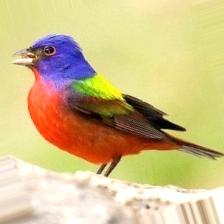
\includegraphics[width=0.24\textwidth]{aug1.jpeg}
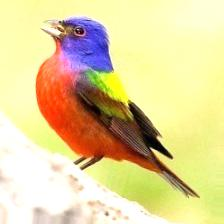
\includegraphics[width=0.24\textwidth]{aug2.jpeg}
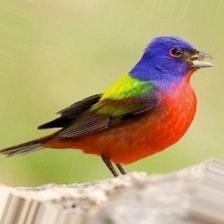
\includegraphics[width=0.24\textwidth]{aug3.jpeg}
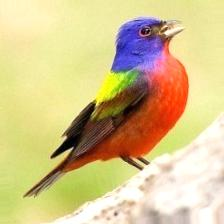
\includegraphics[width=0.24\textwidth]{aug4.jpeg}
\caption{Rotation, shearing, flipping and brightness adjustments applied to a picture}
\end{figure}




\subsection{Mixup}

As mentioned under Related Work, mixup creates virtual training example by combining two images by 

\begin{align*}
&\tilde{x} = \lambda x_i + (1-\lambda) x_j, \qquad \text{where $x_i$, $x_j$ are input vectors} \\
&\tilde{y} = \lambda y_i + (1-\lambda) y_j, \qquad \text{where $y_i$, $y_j$ are one-hot endoced labels}
\end{align*}

where $\lambda \sim$ Beta$(\alpha, \alpha)$.
 This distribution seems like a 
reasonable chioce since it has the right support and the Beta-distribution is the most natural distribution to
consider when working with probabilities. The Beta$(\alpha, \alpha)$-distribution is also symmetric around $0.5$, which may be 
a desireable property, however this should not matter since we combine our randomly drawn examples with weights $\lambda$ and $1-\lambda$ and 
it would not matter if, for example $\lambda = 0.2$ or $\lambda = 0.8$ since it would yield the same two weights, but in different order, but 
since our examples are randomly drawn the order of the weight should not have an impact. 

When reading about mixup, the use of the Beta-distribution is usually taken for granted, however, there are many other distribution which 
could be considered since the only requirement is that the distribution satisfy $\lambda \in [0,1]$. We will therfore not only consider the 
Beta-distribution. 

WRITE ABOUT OTHER DISTRIBUTION(S) (logit-normal)

We will also consider only performing mixup on the input vectors of the training images but letting $\tilde{y}$ keep the label of the exemple 
with the highest weight. That is,

\begin{align*}
\tilde{y} = I_{\{ \lambda \leq 0.5 \}} y_i + (1-I_{\{ \lambda \leq 0.5 \}}) y_j, 
\end{align*}

where $I_{\{ \lambda \leq 0.5 \}} = 1$ if $\lambda \leq 0.5$ and $0$ otherwise.

\begin{figure}[!htb]
	\minipage{0.32\textwidth}
	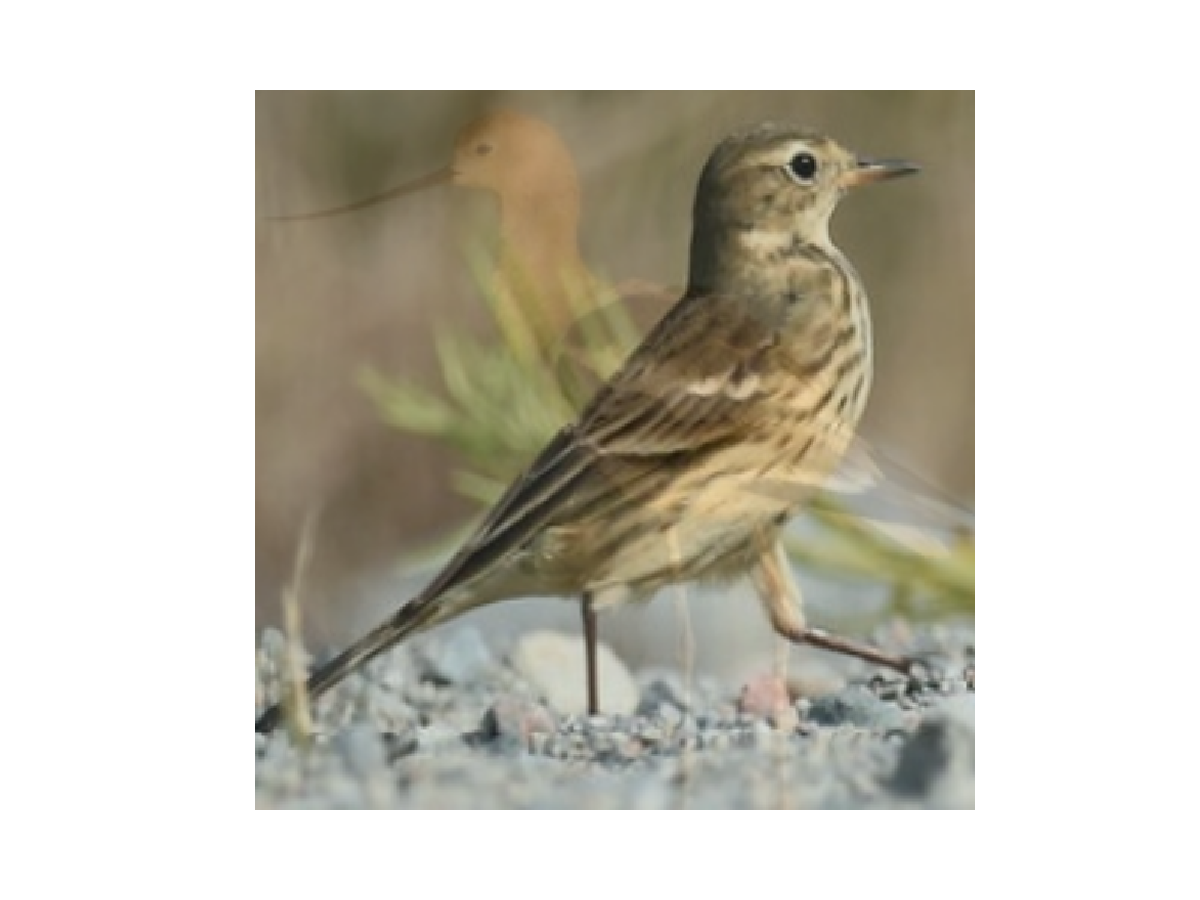
\includegraphics[trim=3cm 2cm 3cm 3cm, width=\linewidth]{mixup1.pdf}
	\endminipage\hfill
	\minipage{0.32\textwidth}
	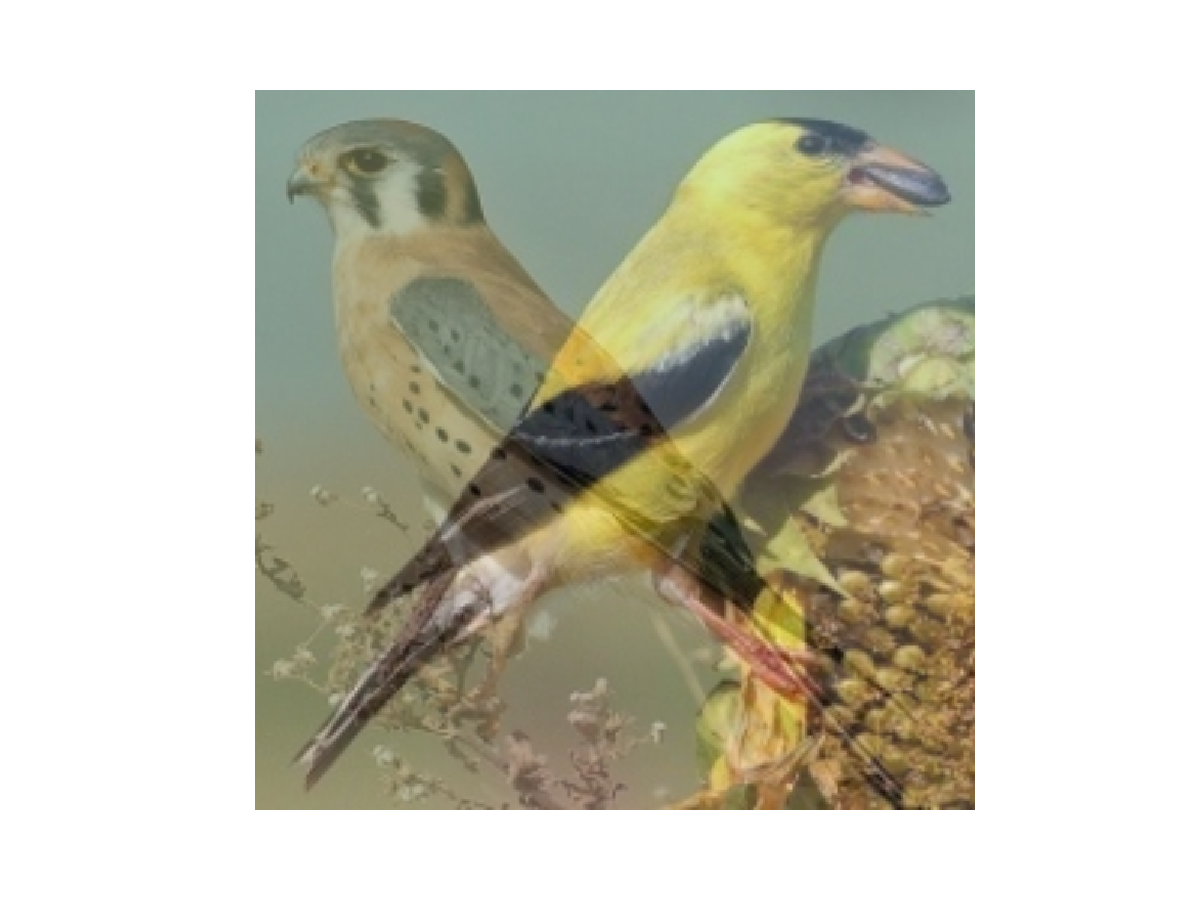
\includegraphics[trim=3cm 2cm 3cm 3cm, width=\linewidth]{mixup2.pdf}
	\endminipage\hfill
	\minipage{0.32\textwidth}%
	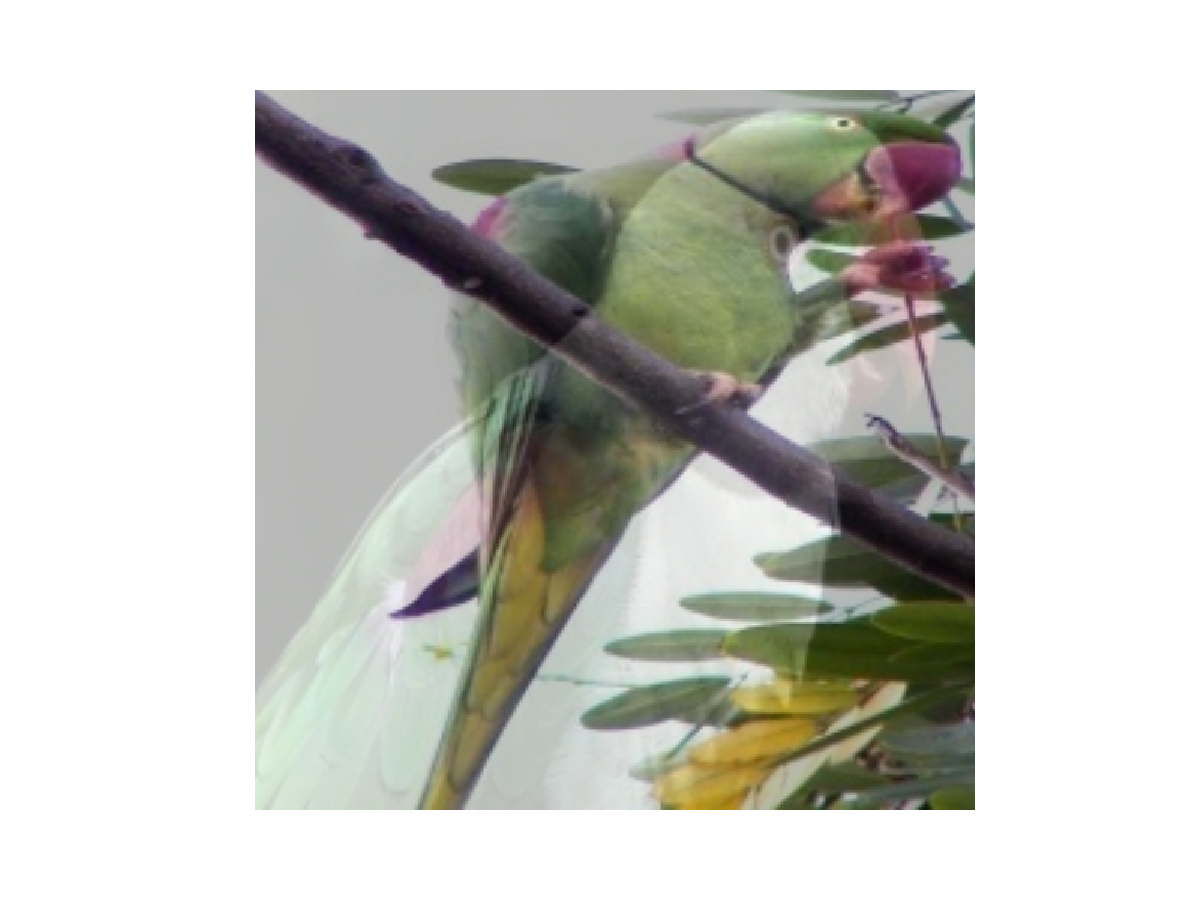
\includegraphics[trim=3cm 2cm 3cm 3cm, width=\linewidth]{mixup3.pdf}
	\endminipage
	\caption{Three examples of mixup performed om images of different bird species.}
\end{figure}

\subsection{Random Erasing}

Random erasing is a bit similar to Mixup in the sense that it aim at confusing the network a little, hopefully just enough for it to see the more general traits and overfit and memorize less.

We wish to compare Mixup with Random Erasing and see which has the strongest effect on the birds dataset and if they may be used together.

We have chosen to let the box be different nuances of gray, so that the network does not focus on the color. Random colorization of the pixels in the box has proven to often be the most successful, however we though that in this dataset using more colors might confuse, and also gray(white-black) was easier to implement.

We have constrained the box to cover between 10 and 20 percent of the image and let the probability of a box being placed be 0.3. 

\begin{figure}[h]
	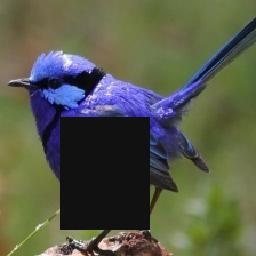
\includegraphics[width=0.24\textwidth]{re1.jpeg}
	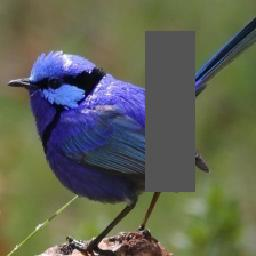
\includegraphics[width=0.24\textwidth]{re2.jpeg}
	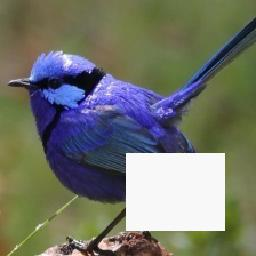
\includegraphics[width=0.24\textwidth]{re3.jpeg}
	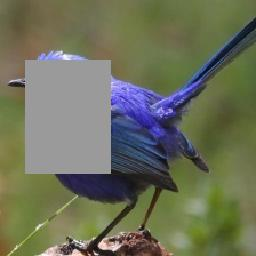
\includegraphics[width=0.24\textwidth]{re4.jpeg}
	\caption{4 different random erasings for an image}
\end{figure}

\subsection{Fourier Transformation}

The 2D Fourier transform is used in for instance in image compression and gave us the idea of the possibility using it in deep learning and image classification. 
The 2D fast Fourier transform take our image, with size $[224 \times 224 \times 3]$, as input and return a complex matrix of the same size. From this output we can now get the amplitudes 
by taking the absolute value of each element in the matrix and the phase angles by computing $arctan(y, x)$, where $x$ is the real part and $y$ is the complex part. 
An interesting property is that the phase angels are more important than the amplitudes and contain more information necessary to recreate the image again. 
As an example, in Figure 2 the Fourier transform was applied to two images which yielded amplitudes and phase angles respectively. 
The images were then recreated using the amplitudes from the first image and the phase angles from the second image and vise versa. 

\begin{figure}[!htb]
	\centering
	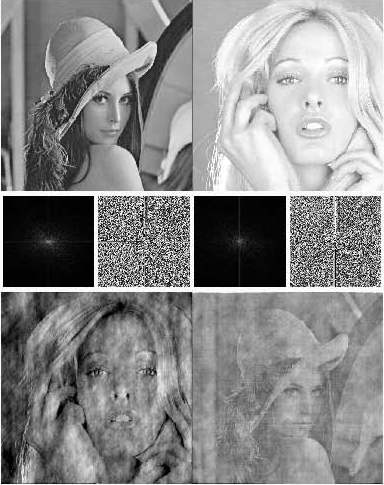
\includegraphics[scale = 0.25]{fourier.jpg}
	\caption{Example of recreation of images using amplitudes and phase angles of the Fourier transformation. 
	Bottom left image use the amplitudes from the first image and the phase angels from the second image and 
	bottom left image use the phase angles from the first image and the amplitudes from the second image}
\end{figure}

Using this as the inspiration we wanted to see if it is true that the phase angles contain more essential information about the image by image classification on the amplitudes 
and phase angels respectively to see if our hypothesis of higher accuracy on the phase angles is satisfied or not. 

Initially we had no expectations that using the fourier transform as augmentation would yield an increase the classification accuracy compared to using 
the raw data, however we thougt it would be an interesting experiment. 
In Figure 3 we can see an example of the Fourier transformation on one of the images in our dataset. 

\begin{figure}[!htb]
	\minipage{0.4\textwidth}
	\raggedleft
	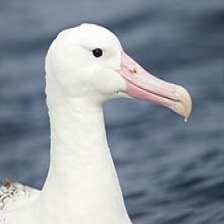
\includegraphics[scale=0.30]{fourier1}
	\endminipage
	\minipage{0.32\textwidth}
	\raggedleft
	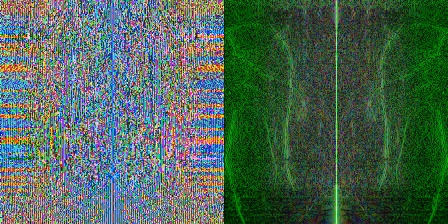
\includegraphics[trim=0cm 0cm 0cm 0cm, scale=0.30]{fourier2}
	\endminipage
	\caption{Left: Original image. Middle: Phase angles. Right: Amplitudes.}
\end{figure}

\subsection{Underlying CNNs}

In order to examine the effects of our data augmentation methods we wanted to observe them for some different networks. Due to time we were only able to focus on two. Below are the networks we examined.

\begin{enumerate}[(i)]
 \item Basic CNN
 \item ResNet50 trained on ImageNet
\end{enumerate}

For the Basic CNN the structure of the layers are shown in Figure 6.

We have chosen CNNs since they have shown to perform good, sometimes extremely good, on computer vision tasks. BatchNormalization has been a necessity in order to manage the gradients and to keep the network stable. We have further used dropout to avoid overfitting which we have anticipated to encounter, both considering the fact that we have several million parameters and also that we will try the network on subsets with very few training examples. Further explanations about the exact order and parameters are provided in the experiments section.

We also chose to use ResNet50 in order to observe how the data augmentations techniques alter the performance in the case of transfer learning.

\begin{figure}[H]
	\centering
	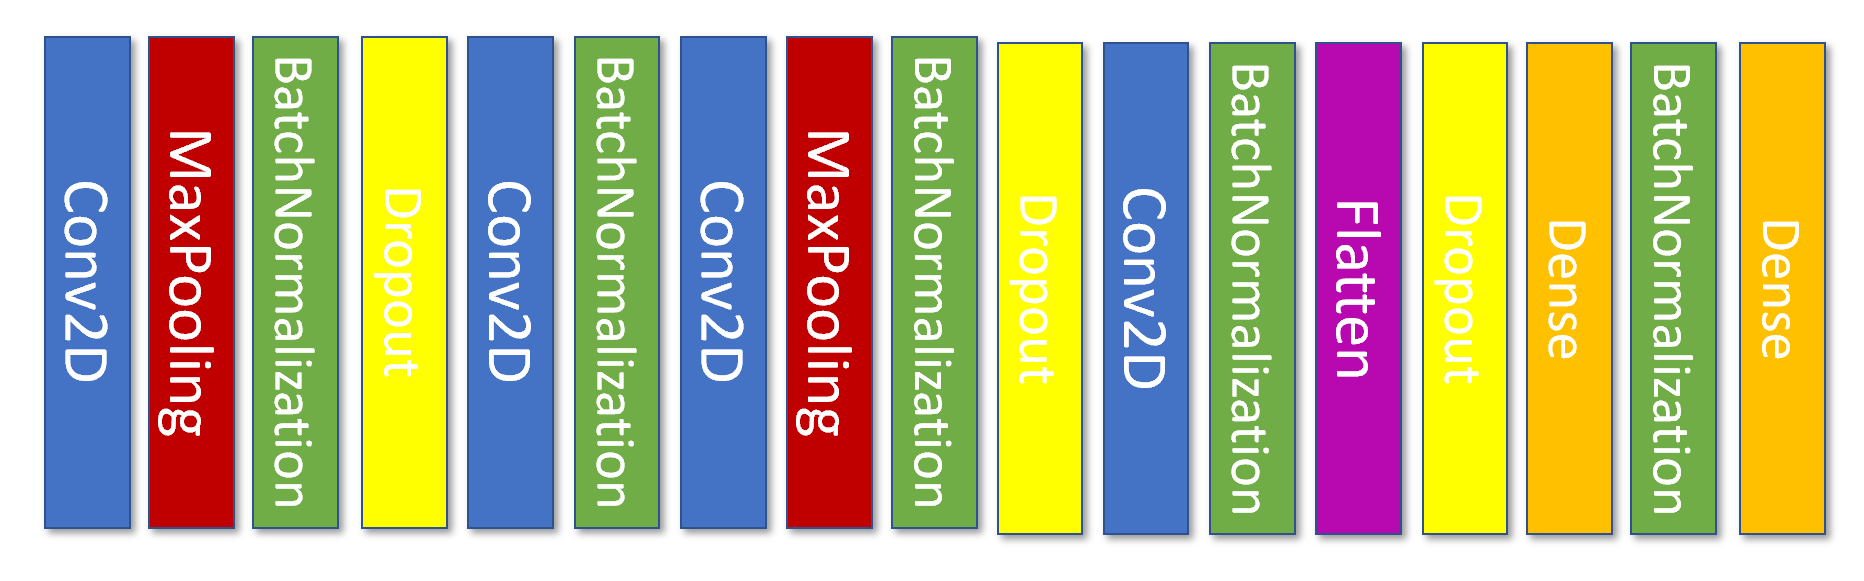
\includegraphics[width=0.9\textwidth]{conv.PNG}
	\caption{Layers of the basic CNN}
\end{figure}

\section{Experiments}

1.5-2.5 pages

\textit{Discuss the experiments that you performed todemonstrate  that  your  approach  solves  the  problem.   The  exact  ex-periments will vary depending on the project, but you might comparewith previously published methods, perform an ablation study to de-termine the impact of various components of your system, experimentwith different hyperparameters or architectural choices, use visualization  techniques  to  gain  insight  into  how  your  model  works,  discuss common failure modes of your model, etc.  You should include graphs,tables, or other figures to illustrate your experimental results.}	

\subsection{Basic Augmentation}
In table 1-3 the results are shown for the runs with all three CNNs on all subsets(except the full datasets is which is excluded since the medium ones have performed very well already) with and without data augmentations. For ResNet where the Small datasets performed very well did not run anything for the Medium size. Recall that there are the same number of species in all datasets(15), what differs is the number of training images(excluding augmentations) for each species(5 or 50).

For our basic CNN and ResNet we can see a great gain in accuracy when applying data augmentations. The difference is the biggest for the basic CNN, but improvements for already good performing networks are hard earned and it is really good that such improvements can be made for such a good performing network with such little effort. 

The basic CNN had quite some problems with the RandomSmall dataset and seems to overfit, here the augmentations made the most difference. The ResNet did not have such problems, maybe because it is pretrained or was better att spotting the relevant parts. The ResNet also perform more evenly across different datasets. It would have been interesting to test ResNet without pretraining, but that was far too time consuming for this project.

It should be said that each combination have only been run once and we do not know anything about the standard deviation of the estimates. It would also have been desirable to try out different randomized selections of species.

\begin{table}[H]
	\caption{Basic CNN and Basic Augmentations}
	\label{sample-table}
	\centering
	\begin{tabular}{lllll}
		\toprule
		Data & Loss No Aug & Loss Basic Aug & Acc No Aug& Acc Basic Aug \\
		\midrule
		RandomSmall  & 6.03 & 3.4 & 0.13 & 0.47 \\
		RandomMedium & 1.81 & 1.01& 0.65 & 0.79 \\
		BrightSmall  & 2.94 & 2.44& 0.40 & 0.53 \\
		BrightMedium & 0.91 & 4.28& 0.84 & 0.90 \\
		DullSmall    & 4.07 & 4.28& 0.27 & 0.38 \\
		DullMedium   & 1.99 & 0.95& 0.57 & 0.81\\
		\bottomrule
	\end{tabular}
\end{table}

\begin{table}[H]
	\caption{ResNet and Basic Augmentations}
	\label{sample-table}
	\centering
	\begin{tabular}{lllll}
		\toprule
		Data & Loss No Aug & Loss Basic Aug & Acc No Aug(\%)& Acc Basic Aug(\%) \\
		\midrule
		RandomSmall  & 0.44 & 0.32& 0.81 & 0.85 \\
		RandomMedium & 0.08 &     & 0.85 &      \\
		BrightSmall  & 0.70 & 0.49& 0.79 & 0.84 \\
		BrightMedium & 0.08 &     & 0.99 &      \\
		DullSmall    & 0.46 & 0.34& 0.83 & 0.89 \\
		DullMedium   & 0.10 &     & 0.99 &      \\
		\bottomrule
	\end{tabular}
\end{table}



\begin{table}[H]
	\caption{MobileNet and Basic Augmentations}
	\label{sample-table}
	\centering
	\begin{tabular}{lllll}
		\toprule
		Data & Loss No Aug & Loss Basic Aug & Acc No Aug(\%)& Acc Basic Aug(\%) \\
		\midrule
		RandomSmall  & 10.91&38.78& 0.37 &0.35  \\
		RandomMedium & 7.02 &     & 0.59 &      \\
		BrightSmall  & 22.43&51.06& 0.37 &0.3   \\
		BrightMedium & 17.20&     & 0.37 &      \\
		DullSmall    & 6.10 &47.69& 0.54 &0.3   \\
		DullMedium   & 22.13&     & 0.14 &      \\
		\bottomrule
	\end{tabular}
\end{table}

As the Random datasets perform very similarly to the Dull ones we continue only with the Bright- and Dull subsets in our further experiments and only run one test on the ResNet which performs very evenly. 

\subsection{MixUp}

In order to examine the effects of MixUp we created our own data generator which used two copies of our main data generator and combined the generated images in order to create the MixUp images as displayed in Figure 2.

In Table X below we showcase the results of a variety of parameter combinations for MixUp on the basic CNN. Note that the first row indicates the training without MixUp.
\begin{table}[H]
	\caption{Basic CNN and MixUp with a Beta distribution}
	\label{sample-table}
	\centering
	\begin{tabular}{lllll}
		\toprule
		Parameter & Label & Accuracy (\%) \\
		\midrule
		 - & - & 64.59  \\
		 0.2 & Majority & 58.29 \\
		 0.2 & Fractional & 54.17 \\ 
		 0.5 & Majority & 54.63 \\
		 0.5 & Fractional & 53.54 \\
		\bottomrule
	\end{tabular}
\end{table}

Below is an alternate approach to MixUp where we instead of the classical Beta distribution implement a Logit-Normal distribution.

\begin{table}[H]
	\caption{Basic CNN and MixUp with a Logit-Normal distribution}
	\label{sample-table}
	\centering
	\begin{tabular}{lllll}
		\toprule
		Parameter & Label & Accuracy (\%) \\
		\midrule
		 - & - & 64.59  \\
		 0.2 & Majority & 50.14 \\
		 0.2 & Fractional & 48.35 \\ 
		 0.5 & Majority & 56.84 \\
		 0.5 & Fractional & 53.54 \\
		\bottomrule
	\end{tabular}
\end{table}

The Logit-Normal distribution does not seem to produce results that are on par with the classical Beta distribution.

\begin{table}[H]
	\caption{ResNet50 and MixUp with a Beta distribution}
	\label{sample-table}
	\centering
	\begin{tabular}{lllll}
		\toprule
		Parameter & Label & Accuracy (\%) \\
		\midrule
		 - & - & 94.78  \\
		 0.2 & Majority & 92.14 \\
		 0.2 & Fractional & 82.21 \\ 
		 0.5 & Majority & 54.63 \\
		 0.5 & Fractional & 53.54 \\
		\bottomrule
	\end{tabular}
\end{table}

\subsection{Random Erasing}

\subsection{The Fourier Transform}

In order to examine which components from the Fourier transform, that is the angles, the amplitudes or the combination of them, that generated the best results we examined their respective performances using the basic CNN architechture. The network was trained for 20 epochs in each experiment using a batch size of 100 and a learning rate of 0.01 in combination with momentum and some decay. It should be noted that the training time increases drastically when taking both the angles and the amplitudes into account as the dimensions of the input increases.

\begin{table}[H]
  \caption{Basic CNN and Fourier Transform}
  \label{sample-table}
  \centering
  \begin{tabular}{ll}
    \toprule
    Data & Accuracy full dataset(\%) \\
    \midrule
    Raw Images  & 64.59 \\
    Fourier Angles & 28.84   \\
    Fourier Amplitudes & 48.42 \\
    Fourier Angles \& Amplitueds & 47.42 \\
    \bottomrule
  \end{tabular}
\end{table}

For the basic CNN it seems as if using only the amplitudes generated the highest accuracy which seems to contradict what we initially thought about the phase angles containing more information about the content of the image. In all, it seems as if the Fourier transform of the input data is not a valid method in order to improve the performance of a CNN, or at least not in the case of our bird data. An interesting extension could be to apply this method to different datasets with more internal variety, such as for example CIFAR 100.

\medskip

Due to computational constraints as well as the quite clear results from the performance on the Basic CNN we did not evaluate the effects of the Fourier transform on other datasets as well as neither on MobileNet nor ResNet50. A major reason for this is that the pre-trained weights from ImageNet are in no way compatible with our angles and amplitudes which would imply a complete re-training using the base architechtures.

\section{Conclusions}

0.25-0.5 pages

\textit{Summarize your key results - what have you learned? Suggest ideas for future extensions or new applications of your ideas.}

What we have implemented is \textit{input mixup} where we do all augmentation before training and input the images in the network after performing mixup, however https://arxiv.org/pdf/1806.05236.pdf 
suggest a new algorithm called \textit{manifold mixup} where mixup is performed at an intermediate layer or final layer in the network. In an intermediate layer 
the feature spaces are more aligned than that of the input and it is suggested that mixup will produce better augmented data if the mixup is performed on this layer. Therefore, this would be 
a natural possible future extention to this project. 


\section*{References}

Shorten \& Khoshgoftaar (2019) A survey on Image Data Augmentation for Deep Learning, \textit{Journal of Big data 6}

Zhang et al (2018) Mixup: Beyond Empirical risk minimization \textit{ICLR conference paper 2018}

Exempel:
\medskip

\small

[1] Alexander, J.A.\ \& Mozer, M.C.\ (1995) Template-based algorithms for
connectionist rule extraction. In G.\ Tesauro, D.S.\ Touretzky and T.K.\ Leen
(eds.), {\it Advances in Neural Information Processing Systems 7},
pp.\ 609--616. Cambridge, MA: MIT Press.

\section{info (ska ej vara med i rapporten)}

-Total 6-8 sidor inkl referenser och appendix


\end{document}
